\documentclass[12pt,a4paper,titlepage]{article}
\usepackage[latin1]{inputenc}
\usepackage{amsmath}
\usepackage{amsfonts}
\usepackage{amssymb}
\usepackage{braket}
\usepackage{graphicx}
\usepackage{subcaption}
\usepackage{array}
\usepackage{pbox}


\author{Tobias G\"oppel and Sophia Kronthaler}
\title{Theoretical Practical Course in Computational Physics}
\begin{document}

\maketitle

\newpage
\tableofcontents
\newpage


\section{Monte Carlo (MC) integration method} 

The Monte Carlo integration method is quite similar to the Riemann integration method with the subtle difference that one chooses the $x_i$s randomly. This leads to the following approximative formula for the integral:

\begin{equation}
I = \frac{b-a}{N} \sum_{i=0}^{N-1} f(x_i) \xrightarrow{N\rightarrow \infty} \int_a^b\! f(x)\, \mathrm{dx}
\end{equation}
												

We can estimate the integral of the function f by:

\begin{equation}
\int_a^b\! f(x),\mathrm{dx} \approx I \pm Error = V \braket{f} \pm V \sqrt{\frac{\braket{f^2}-\braket{f}^2}{N}} 
\end{equation}

Of course we do not know the standard deviation of f but we can approximate it "on the flight" when performing the Monte Carlo integration. In our program, we assume that the desired accuracy is
reached, when:
\[accuracy \geq \frac{\sqrt{\frac{\braket{f^2}-\braket{f}^2}{N}}}{\braket{f}} \]


As one can see, the error decreases with $\sim \frac{1}{\sqrt{N}}$.
To get an more detailed idea of what determines the error, we should notice that the individual function values at random points $x_i$ one the x-axis are themselvs random numbers.The Integrand, being sum of random numbers is a random number too. The distribution of the integrated values approaches a Gaussian. By using the central limit theorem it can be shown that the following expression holds:

\begin{equation}
\sigma^2(I_N) = \frac{V^2}{N} \int_V \!(f(x) - \braket{f})^2 \mathrm{dx}=\frac{V^2}{N}\sigma^2(f)
\end{equation}

This leads to the important conclusion that the variance of $I_N$ does not depend only on the quantity of random points $N$, but also on the volume $V$ and the variance of the function $\sigma^2(f)$.
To show this characteristic we define the ratio $\rho$.

\[\rho = \frac{N}{V^2}\frac{\sigma^2(I_N)}{\sigma^2(f)}\]
\newpage


\begin{figure}
\centering
\caption{$f(x)=x$, volume: $[-1,1]$, ratio: 1.051}
	\begin{minipage}[b]{\linewidth}
		\centering
		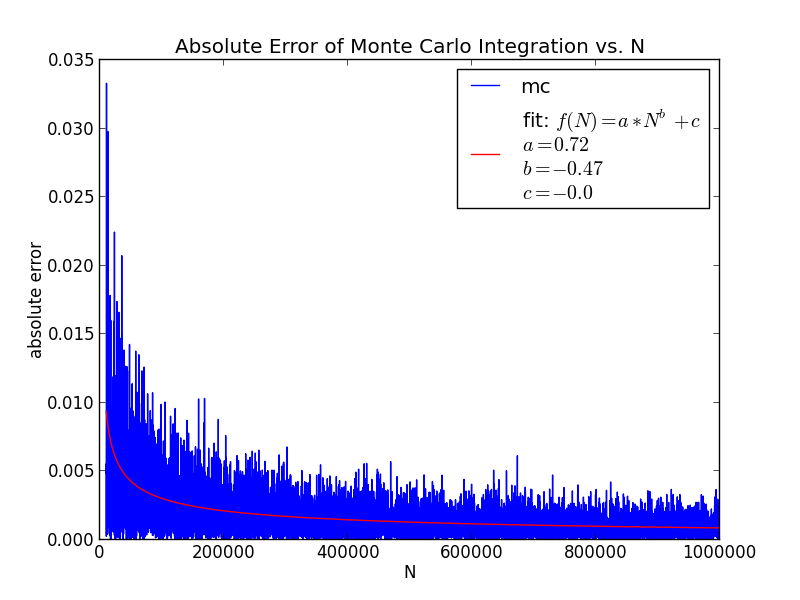
\includegraphics[width=\linewidth]{Plots/linear}
	\end{minipage}
	\begin{minipage}[b]{\linewidth}
		\centering
		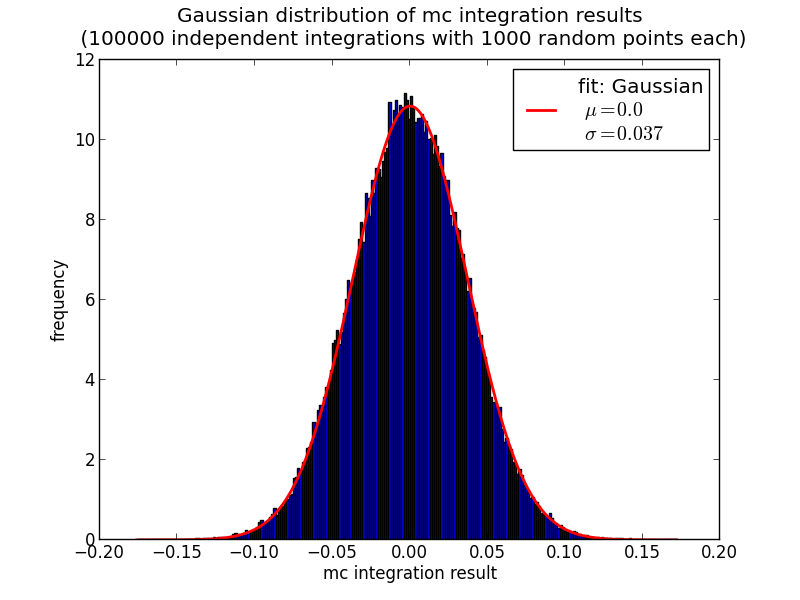
\includegraphics[width=\linewidth]{Plots/linearhist}
	\end{minipage}
\label{fig:linear}
\end{figure}
\begin{figure}
	\centering
	\caption{$f(x)=x^2$, volume: $[-1,1]$, ratio: 1.043}
	\begin{minipage}[b]{\linewidth}
		\centering
		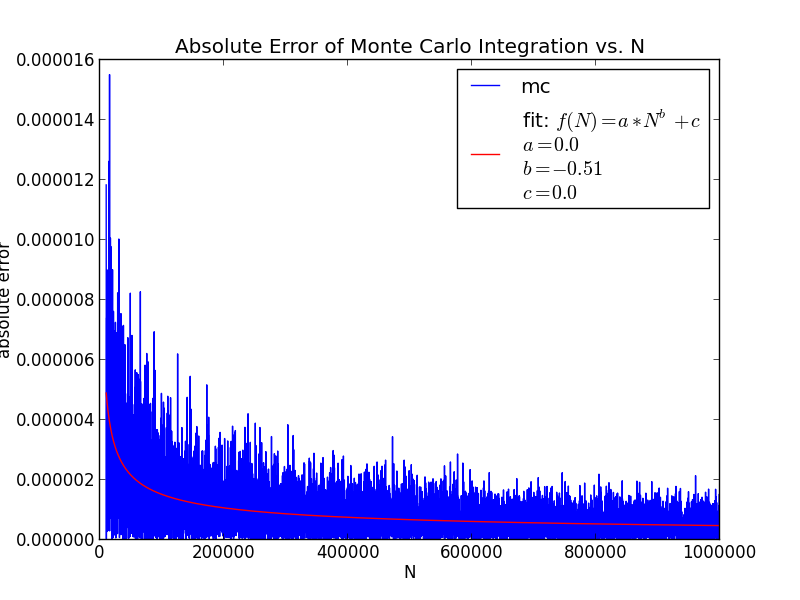
\includegraphics[width=\linewidth]{Plots/quadratisch}
	\end{minipage}
	\begin{minipage}[b]{\linewidth}
		\centering
		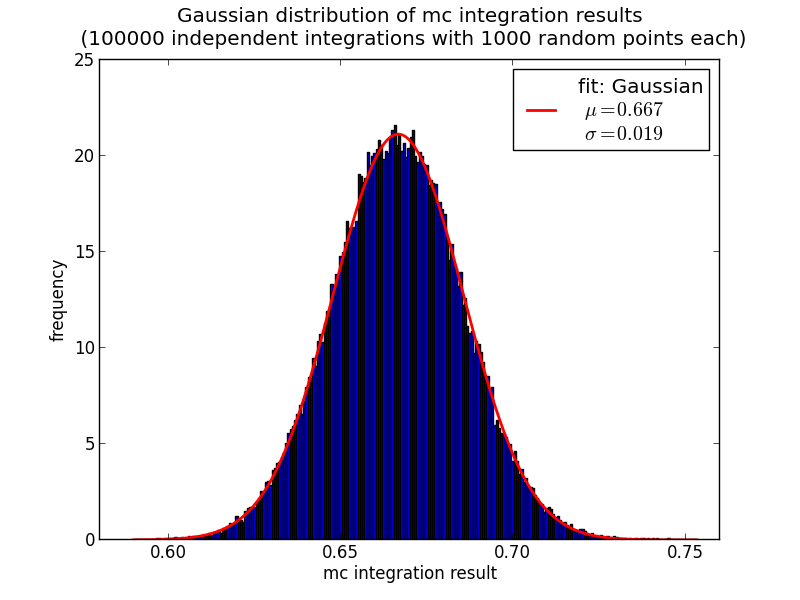
\includegraphics[width=\linewidth]{Plots/histQuadratisch}
	\end{minipage}
	\label{fig:linear}
\end{figure}
\begin{figure}
	\centering
	\caption{$f(x)=x^5$, volume: $[-1,1]$, ratio: 0.951, (the fit function failed to find the correct fit paramters for the Gaussian)}
	\begin{minipage}[b]{\linewidth}
		\centering
		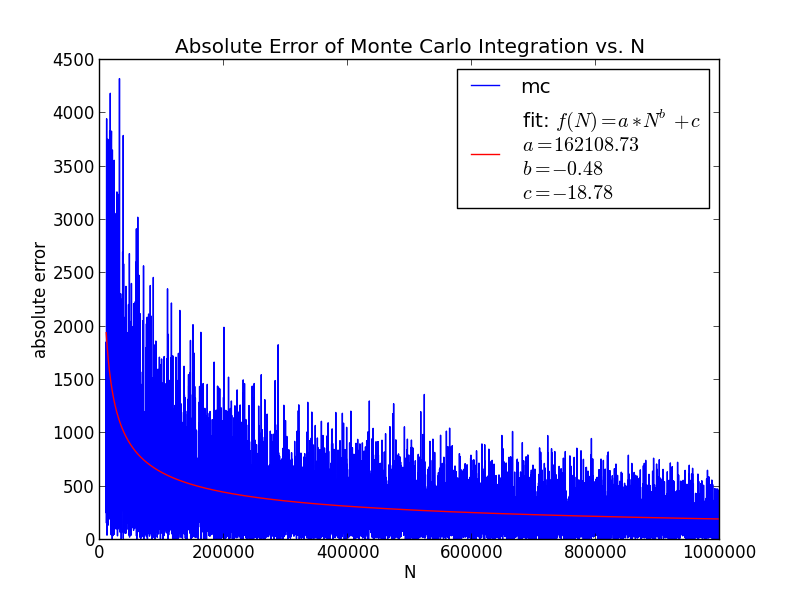
\includegraphics[width=\linewidth]{Plots/x5}
	\end{minipage}
	\begin{minipage}[b]{\linewidth}
		\centering
		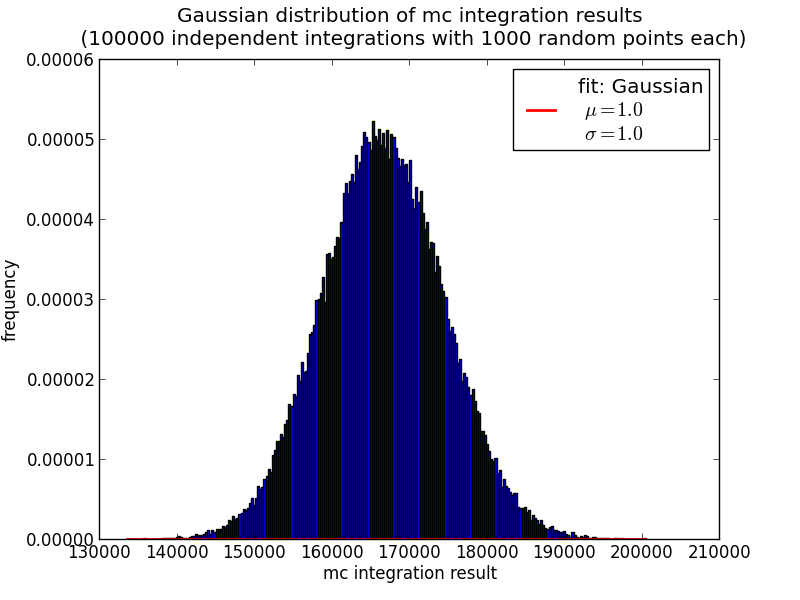
\includegraphics[width=\linewidth]{Plots/x5_HIST}
	\end{minipage}
	\label{fig:linear}
\end{figure}
\begin{figure}
	\centering
	\caption{$f(x)=exp(x)$, volume: $[-1,1]$, ratio: 0.932}
	\begin{minipage}[b]{\linewidth}
		\centering
		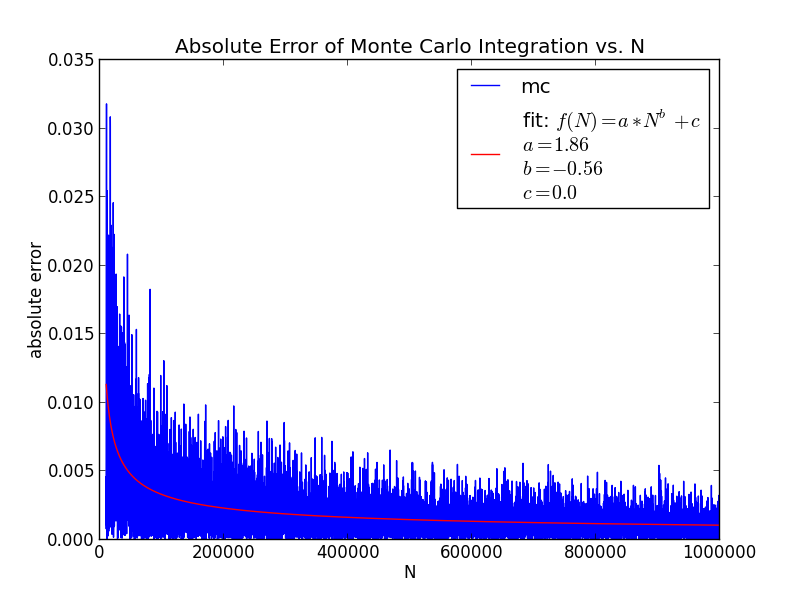
\includegraphics[width=\linewidth]{Plots/eFunktion}
	\end{minipage}
	\begin{minipage}[b]{\linewidth}
		\centering
		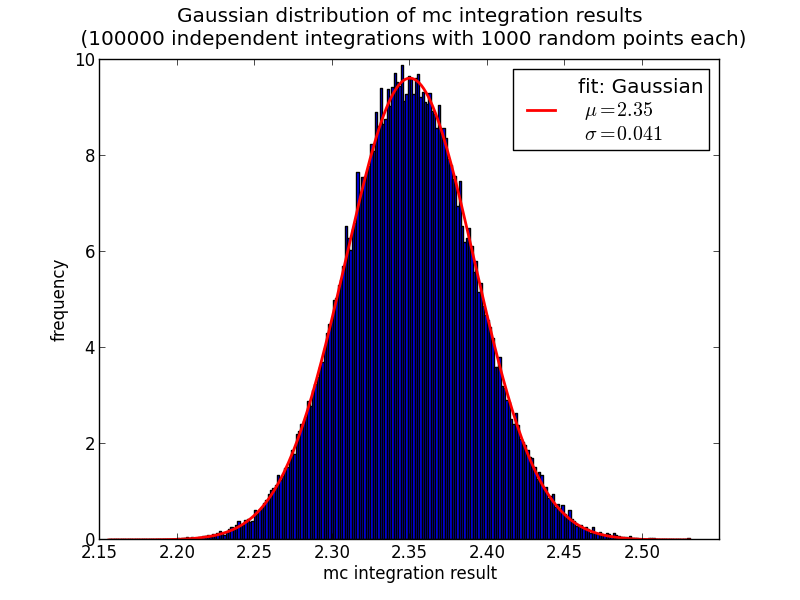
\includegraphics[width=\linewidth]{Plots/eFunktionHist}
	\end{minipage}
	\label{fig:linear}
\end{figure}
\begin{figure}
	\centering
	\caption{$f(x)=sin(x)$, volume: $[0,2\pi]$, ratio: 1.085}
	\begin{minipage}[b]{\linewidth}
		\centering
		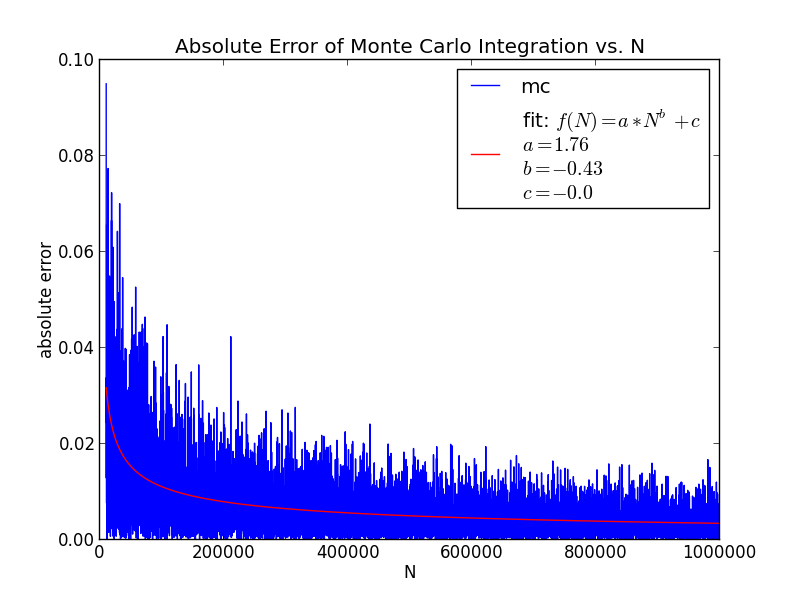
\includegraphics[width=\linewidth]{Plots/sin}
	\end{minipage}
	\begin{minipage}[b]{\linewidth}
		\centering
		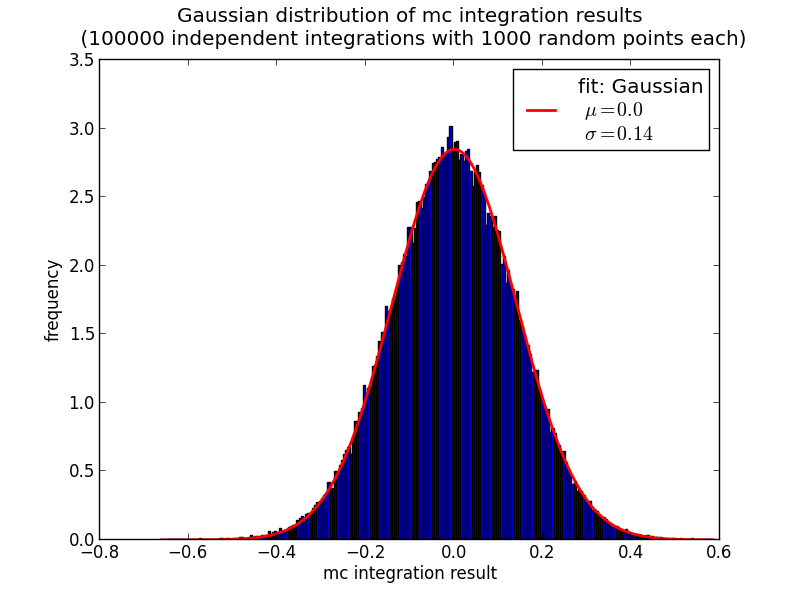
\includegraphics[width=\linewidth]{Plots/sin_hist}
	\end{minipage}
	\label{fig:linear}
\end{figure}

\newpage
\section{Ising Model}

The Ising model is a well known toy model for ferromagnetism, for that reason it will not be explained in detail here.
The Hamiltonian for a predefined spin configration $\{c\}$ is given by:
 \[H(\{c\})= - \frac{1}{2}\sum_{i=0}^{N-1} \sum_{j=0}^{N-1} J_{ij} s_i s_j - B \sum_{i=0}^{N-1}s_i\]

$J_{ij}$ (coumpling term) determines the strength of the force exerted in an interaction of neighbouring spins. It depends on the sign of the coupling constant whether the ground state is ordered or disordered. 
\[J_{ij} > 0 \text{the interaction is called ferromagnetic with an ordered GS: } E_0=-NJ\]
\[J_{ij} < 0 \text{the interaction is called anti-ferromagnetic with an disordered GS: } E_0=+NJ\]
In this model we solely consider nearest neighbours interaction with periodic boundary conditions.
With an occupation propability for a specific spin configuration of
\[P(\{c\}) \sim \exp[-\beta H(\vec{S})] \text{with } \beta = \frac{1}{k_B T}\]
one can compute the observables listed below:\newline

\textbf{1d withou magnetic field (per spin):}
\begin{align*}
&\braket{u} = \sum_{\{c\}}H(\{c\})P(\{c\}) = -J \tanh(\beta J)\\
&\braket{c} = k_B(\beta J)^2[1-\tanh^2(K)]\\
&\braket{m} = 0 
\end{align*} 


\textbf{1d with magnetic field (per spin):}
\begin{align*}
&\braket{m} = \frac{\sinh(h)}{\sqrt{\sinh^2(h) + \exp(-4\beta J) }}\\
&\braket{\chi}=\beta \cosh(h) \frac{\exp(-4J\beta)}{(\sinh(h)+\exp(-4J\beta))^{\frac{3}{2}}}
\end{align*}


To obtain the exact solutoin for the 2d Ising Model is a story in itself.\footnote[1]{We recommend the Advanced Statisical Physics Script,
\newline Prof. Dr. Ulrich Schollwoeck, Chapter 7}







\section{Metropolis Algorithm}

The aim ist to generate configurations of Ising systems in thermal equilibrium at a given temperature. The standard method, the Metropolis Algorithm, of acquiring these sample configurations is actually a modified Monte Carlo scheme 'Instead of choosing configurations randomly and then weighting them, we choose configurations with a probability $P\sim \exp(-\frac{E}{k_b T}))$ and weight them evenly.'\cite{metropolis}\newline
The following steps illustrate the Metropolis method:\newline
In the beginning, select some initial spin configuration $\{c^0\}$ and compute its energy $E_0 = H(\{c^0\})$.
Then:


\begin{enumerate}
\item Randomly select one spin $s_i$ of the configuration $\{c\}$
\item Flip $s_i \rightarrow -s_i$ to obtain $\{c^n\} \rightarrow \{c^*\}$
\item Compute the energy $E_*=H(\{c^*\})$ for the new configuration
\item If $E_*\leq E_n$ accept the new configuration $\{c^{n+1}\} = \{c^*\}$
\item Else accept the new configuration with a propability of $\exp(-\beta \bigtriangleup E)$
\item If finally rejected duplicate old configuration $\{c^{n+1}\} = \{c^n\}$
\item Compute $E_{n+1} = H(\{c^{n+1}\})$
\end{enumerate}

To speed up the simulation, we modified these steps by avoiding exponentations and total energy evaluations inside the metropolis loop.
On that account we calculate the 'acceptance-' or 'weightening-cases' in advance by hand and merely check whichever takes place.
In the beginning, select some initial configuration $\{c^0\}$, compute its energy $E_0 = H(\{c^0\})$, its energy changes by $\bigtriangleup E$ by fliiping a spin and its weights $P(\bigtriangleup E)$.
\begin{enumerate}
\item Randomly select one spin $s_i$ of the configuration $\{c\}$
\item Check which case is applicable
\item If it's an 'acceptance-case', flip the spin and calculate the new energy by $E_{n+1} = E_n + \bigtriangleup E$
\item Else accept the new configuration with the applicable propability saved in the weights
\end{enumerate}



\begin{table}[h]
\centering
\caption{ 1D without magnetic field}

\begin{tabular}{|>{$}c<{$}|>{$}c<{$}|>{$}c<{$}|}
\hline 
\text{case} & \bigtriangleup \text{E} & \text{weight} \\ 
\hline 
+++ \rightarrow +-+ & +8J & exp(-8\beta J) \\ 
\hline 
+-+ \rightarrow +++ & -4J & \text{accept} \\ 
\hline 
+-- \rightarrow ++- & 0 & \text{accept}\\
\hline
\end{tabular} 
\end{table}


\begin{table}[h]
\centering
\caption{ 1D with magnetic field (h field is +)}

\begin{tabular}{|>{$}c<{$}|>{$}c<{$}|>{$}l<{$}|}
\hline 
\text{case} & \bigtriangleup \text{E} & \text{weight} \\ 
\hline 
+++ \rightarrow +-+ & 4J +2h & exp(-4\beta J - 2\beta h) \\ 
\hline 
--- \rightarrow -+- & 4J-2h & \text{ if } 4J > 2h \;:\exp(-4\beta J +2\beta h)\; else\; : \text{accept} \\ 
\hline 
+-+ \rightarrow +++ & -4J-2h & \text{accept}\\
\hline
-+- \rightarrow --- & -4J+2h & \text{ if } 4J < 2h \;:\exp(4\beta J -2\beta h)\; else\; : \text{accept}\\
\hline
++- \rightarrow +-- & 2h & \exp(-2\beta h)\\
\hline
--+ \rightarrow -++ & 2h & \text{accept}\\
\hline
\end{tabular} 
\end{table}


\begin{table}[h]
\centering
\caption{ 2D without magnetic field}

\begin{tabular}{|>{$}c<{$}|>{$}c<{$}|>{$}c<{$}|}
\hline 
\text{case} & \bigtriangleup \text{E} & \text{weight} \\ 
\hline 
\parbox[4em]{1cm}{$+++$\\$+++$\\$+++$} \longrightarrow \pbox{20cm}{$+++$\\$+-+$\\$+++$} & 8J & exp(-8\beta J) \\ 
\hline 
\parbox[4em]{1cm}{$+++$\\$+++$\\$++-$} \longrightarrow \pbox{20cm}{$+++$\\$+-+$\\$++-$} & 4J & exp(-4\beta J) \\ 
\hline 
\parbox[4em]{1cm}{$+++$\\$++-$\\$+-+$} \longrightarrow \pbox{20cm}{$+++$\\$+--$\\$+-+$} & 0 & \text{accept} \\ 
\hline
\parbox[4em]{1cm}{$+++$\\$-+-$\\$+-+$} \longrightarrow \pbox{20cm}{$+++$\\$---$\\$+-+$} & -4J & \text{accept} \\ 
\hline
\parbox[4em]{1cm}{$+-+$\\$-+-$\\$+-+$} \longrightarrow \pbox{20cm}{$+-+$\\$---$\\$+-+$} & -8J & \text{accept} \\ 
\hline

\end{tabular} 
\end{table}




\newpage
\section{Implementation and Performance}



\begin{thebibliography}{9}


\bibitem{metropolis}

Nicholas Metropolis, Arianna W. Rosenbluth, Marshall N. Rosenbluth, Augusta H. Teller, and Edward
Teller. Equation of state calculations by fast computing machines. The Journal of Chemical Physics, 1953.



\end{thebibliography}




\end{document}